\documentclass[twoside]{book}

% Packages required by doxygen
\usepackage{fixltx2e}
\usepackage{calc}
\usepackage{doxygen}
\usepackage{graphicx}
\usepackage[utf8]{inputenc}
\usepackage{makeidx}
\usepackage{multicol}
\usepackage{multirow}
\PassOptionsToPackage{warn}{textcomp}
\usepackage{textcomp}
\usepackage[nointegrals]{wasysym}
\usepackage[table]{xcolor}

% NLS support packages
\usepackage[french]{babel}

% Font selection
\usepackage[T1]{fontenc}
\usepackage{mathptmx}
\usepackage[scaled=.90]{helvet}
\usepackage{courier}
\usepackage{amssymb}
\usepackage{sectsty}
\renewcommand{\familydefault}{\sfdefault}
\allsectionsfont{%
  \fontseries{bc}\selectfont%
  \color{darkgray}%
}
\renewcommand{\DoxyLabelFont}{%
  \fontseries{bc}\selectfont%
  \color{darkgray}%
}
\newcommand{\+}{\discretionary{\mbox{\scriptsize$\hookleftarrow$}}{}{}}

% Page & text layout
\usepackage{geometry}
\geometry{%
  a4paper,%
  top=2.5cm,%
  bottom=2.5cm,%
  left=2.5cm,%
  right=2.5cm%
}
\tolerance=750
\hfuzz=15pt
\hbadness=750
\setlength{\emergencystretch}{15pt}
\setlength{\parindent}{0cm}
\setlength{\parskip}{0.2cm}
\makeatletter
\renewcommand{\paragraph}{%
  \@startsection{paragraph}{4}{0ex}{-1.0ex}{1.0ex}{%
    \normalfont\normalsize\bfseries\SS@parafont%
  }%
}
\renewcommand{\subparagraph}{%
  \@startsection{subparagraph}{5}{0ex}{-1.0ex}{1.0ex}{%
    \normalfont\normalsize\bfseries\SS@subparafont%
  }%
}
\makeatother

% Headers & footers
\usepackage{fancyhdr}
\pagestyle{fancyplain}
\fancyhead[LE]{\fancyplain{}{\bfseries\thepage}}
\fancyhead[CE]{\fancyplain{}{}}
\fancyhead[RE]{\fancyplain{}{\bfseries\leftmark}}
\fancyhead[LO]{\fancyplain{}{\bfseries\rightmark}}
\fancyhead[CO]{\fancyplain{}{}}
\fancyhead[RO]{\fancyplain{}{\bfseries\thepage}}
\fancyfoot[LE]{\fancyplain{}{}}
\fancyfoot[CE]{\fancyplain{}{}}
\fancyfoot[RE]{\fancyplain{}{\bfseries\scriptsize Généré le Mercredi 30 Mars 2016 14\+:03\+:54 pour To\+Do\+List par Doxygen }}
\fancyfoot[LO]{\fancyplain{}{\bfseries\scriptsize Généré le Mercredi 30 Mars 2016 14\+:03\+:54 pour To\+Do\+List par Doxygen }}
\fancyfoot[CO]{\fancyplain{}{}}
\fancyfoot[RO]{\fancyplain{}{}}
\renewcommand{\footrulewidth}{0.4pt}
\renewcommand{\chaptermark}[1]{%
  \markboth{#1}{}%
}
\renewcommand{\sectionmark}[1]{%
  \markright{\thesection\ #1}%
}

% Indices & bibliography
\usepackage{natbib}
\usepackage[titles]{tocloft}
\setcounter{tocdepth}{3}
\setcounter{secnumdepth}{5}
\makeindex

% Hyperlinks (required, but should be loaded last)
\usepackage{ifpdf}
\ifpdf
  \usepackage[pdftex,pagebackref=true]{hyperref}
\else
  \usepackage[ps2pdf,pagebackref=true]{hyperref}
\fi
\hypersetup{%
  colorlinks=true,%
  linkcolor=blue,%
  citecolor=blue,%
  unicode%
}

% Custom commands
\newcommand{\clearemptydoublepage}{%
  \newpage{\pagestyle{empty}\cleardoublepage}%
}


%===== C O N T E N T S =====

\begin{document}

% Titlepage & ToC
\hypersetup{pageanchor=false,
             bookmarks=true,
             bookmarksnumbered=true,
             pdfencoding=unicode
            }
\pagenumbering{roman}
\begin{titlepage}
\vspace*{7cm}
\begin{center}%
{\Large To\+Do\+List }\\
\vspace*{1cm}
{\large Généré par Doxygen 1.8.7}\\
\vspace*{0.5cm}
{\small Mercredi 30 Mars 2016 14:03:54}\\
\end{center}
\end{titlepage}
\clearemptydoublepage
\tableofcontents
\clearemptydoublepage
\pagenumbering{arabic}
\hypersetup{pageanchor=true}

%--- Begin generated contents ---
\chapter{Index des espaces de nommage}
\section{Liste des espaces de nommage}
Liste de tous les espaces de nommage avec une brève description\+:\begin{DoxyCompactList}
\item\contentsline{section}{\hyperlink{namespace_to_do_core}{To\+Do\+Core} }{\pageref{namespace_to_do_core}}{}
\item\contentsline{section}{\hyperlink{namespace_to_do_core_1_1testing}{To\+Do\+Core\+::testing} }{\pageref{namespace_to_do_core_1_1testing}}{}
\end{DoxyCompactList}

\chapter{Index hiérarchique}
\section{Hiérarchie des classes}
Cette liste d'héritage est classée approximativement par ordre alphabétique \+:\begin{DoxyCompactList}
\item Test\begin{DoxyCompactList}
\item \contentsline{section}{To\+Do\+Core\+:\+:testing\+:\+:To\+Do\+Test}{\pageref{class_to_do_core_1_1testing_1_1_to_do_test}}{}
\end{DoxyCompactList}
\item \contentsline{section}{To\+Do\+Core\+:\+:To\+Do}{\pageref{class_to_do_core_1_1_to_do}}{}
\end{DoxyCompactList}

\chapter{Index des classes}
\section{Liste des classes}
Liste des classes, structures, unions et interfaces avec une brève description \+:\begin{DoxyCompactList}
\item\contentsline{section}{\hyperlink{class_to_do_core_1_1_to_do}{To\+Do\+Core\+::\+To\+Do} }{\pageref{class_to_do_core_1_1_to_do}}{}
\item\contentsline{section}{\hyperlink{class_to_do_core_1_1testing_1_1_to_do_test}{To\+Do\+Core\+::testing\+::\+To\+Do\+Test} }{\pageref{class_to_do_core_1_1testing_1_1_to_do_test}}{}
\end{DoxyCompactList}

\chapter{Index des fichiers}
\section{Liste des fichiers}
Liste de tous les fichiers avec une brève description \+:\begin{DoxyCompactList}
\item\contentsline{section}{/home/latty/\+Prog/\+C\+Make\+\_\+\+Tutorial/chapter\+\_\+4/src/\hyperlink{main_8cc}{main.\+cc} }{\pageref{main_8cc}}{}
\item\contentsline{section}{/home/latty/\+Prog/\+C\+Make\+\_\+\+Tutorial/chapter\+\_\+4/src/\+To\+Do\+Core/\hyperlink{_to_do_8cc}{To\+Do.\+cc} }{\pageref{_to_do_8cc}}{}
\item\contentsline{section}{/home/latty/\+Prog/\+C\+Make\+\_\+\+Tutorial/chapter\+\_\+4/src/\+To\+Do\+Core/\hyperlink{_to_do_8h}{To\+Do.\+h} }{\pageref{_to_do_8h}}{}
\item\contentsline{section}{/home/latty/\+Prog/\+C\+Make\+\_\+\+Tutorial/chapter\+\_\+4/src/\+To\+Do\+Core/unit\+\_\+test/\hyperlink{_to_do_test_8cc}{To\+Do\+Test.\+cc} }{\pageref{_to_do_test_8cc}}{}
\end{DoxyCompactList}

\chapter{Documentation des espaces de nommage}
\hypertarget{namespace_to_do_core}{\section{Référence de l'espace de nommage To\+Do\+Core}
\label{namespace_to_do_core}\index{To\+Do\+Core@{To\+Do\+Core}}
}
\subsection*{Espaces de nommage}
\begin{DoxyCompactItemize}
\item 
 \hyperlink{namespace_to_do_core_1_1testing}{testing}
\end{DoxyCompactItemize}
\subsection*{Classes}
\begin{DoxyCompactItemize}
\item 
class \hyperlink{class_to_do_core_1_1_to_do}{To\+Do}
\end{DoxyCompactItemize}

\hypertarget{namespace_to_do_core_1_1testing}{\section{Référence de l'espace de nommage To\+Do\+Core\+:\+:testing}
\label{namespace_to_do_core_1_1testing}\index{To\+Do\+Core\+::testing@{To\+Do\+Core\+::testing}}
}
\subsection*{Classes}
\begin{DoxyCompactItemize}
\item 
class \hyperlink{class_to_do_core_1_1testing_1_1_to_do_test}{To\+Do\+Test}
\end{DoxyCompactItemize}
\subsection*{Fonctions}
\begin{DoxyCompactItemize}
\item 
\hyperlink{namespace_to_do_core_1_1testing_a8856a84197dfa84ec81d14bd227c2264}{T\+E\+S\+T\+\_\+\+F} (\hyperlink{class_to_do_core_1_1testing_1_1_to_do_test}{To\+Do\+Test}, constructor\+\_\+creates\+Empty\+List)
\item 
\hyperlink{namespace_to_do_core_1_1testing_ad1ff01cd7b75e9ba48225bbde5f1bb2b}{T\+E\+S\+T\+\_\+\+F} (\hyperlink{class_to_do_core_1_1testing_1_1_to_do_test}{To\+Do\+Test}, add\+Task\+\_\+three\+Times\+\_\+size\+Is\+Three)
\item 
\hyperlink{namespace_to_do_core_1_1testing_a8d6cdf71a6d2d85a7d6dc6e4ced72c51}{T\+E\+S\+T\+\_\+\+F} (\hyperlink{class_to_do_core_1_1testing_1_1_to_do_test}{To\+Do\+Test}, get\+Task\+\_\+with\+One\+Task\+\_\+returns\+Correct\+String)
\item 
\hyperlink{namespace_to_do_core_1_1testing_ae6f99ee22a68254ccf5750d1788cd082}{T\+E\+S\+T\+\_\+\+F} (\hyperlink{class_to_do_core_1_1testing_1_1_to_do_test}{To\+Do\+Test}, get\+Task\+\_\+with\+Three\+Tasts\+\_\+returns\+Correct\+String\+For\+Each\+Index)
\end{DoxyCompactItemize}


\subsection{Documentation des fonctions}
\hypertarget{namespace_to_do_core_1_1testing_a8856a84197dfa84ec81d14bd227c2264}{\index{To\+Do\+Core\+::testing@{To\+Do\+Core\+::testing}!T\+E\+S\+T\+\_\+\+F@{T\+E\+S\+T\+\_\+\+F}}
\index{T\+E\+S\+T\+\_\+\+F@{T\+E\+S\+T\+\_\+\+F}!To\+Do\+Core\+::testing@{To\+Do\+Core\+::testing}}
\subsubsection[{T\+E\+S\+T\+\_\+\+F}]{\setlength{\rightskip}{0pt plus 5cm}To\+Do\+Core\+::testing\+::\+T\+E\+S\+T\+\_\+\+F (
\begin{DoxyParamCaption}
\item[{To\+Do\+Test}]{, }
\item[{constructor\+\_\+creates\+Empty\+List}]{}
\end{DoxyParamCaption}
)}}\label{namespace_to_do_core_1_1testing_a8856a84197dfa84ec81d14bd227c2264}


Définition à la ligne 49 du fichier To\+Do\+Test.\+cc.

\hypertarget{namespace_to_do_core_1_1testing_ad1ff01cd7b75e9ba48225bbde5f1bb2b}{\index{To\+Do\+Core\+::testing@{To\+Do\+Core\+::testing}!T\+E\+S\+T\+\_\+\+F@{T\+E\+S\+T\+\_\+\+F}}
\index{T\+E\+S\+T\+\_\+\+F@{T\+E\+S\+T\+\_\+\+F}!To\+Do\+Core\+::testing@{To\+Do\+Core\+::testing}}
\subsubsection[{T\+E\+S\+T\+\_\+\+F}]{\setlength{\rightskip}{0pt plus 5cm}To\+Do\+Core\+::testing\+::\+T\+E\+S\+T\+\_\+\+F (
\begin{DoxyParamCaption}
\item[{To\+Do\+Test}]{, }
\item[{add\+Task\+\_\+three\+Times\+\_\+size\+Is\+Three}]{}
\end{DoxyParamCaption}
)}}\label{namespace_to_do_core_1_1testing_ad1ff01cd7b75e9ba48225bbde5f1bb2b}


Définition à la ligne 53 du fichier To\+Do\+Test.\+cc.

\hypertarget{namespace_to_do_core_1_1testing_a8d6cdf71a6d2d85a7d6dc6e4ced72c51}{\index{To\+Do\+Core\+::testing@{To\+Do\+Core\+::testing}!T\+E\+S\+T\+\_\+\+F@{T\+E\+S\+T\+\_\+\+F}}
\index{T\+E\+S\+T\+\_\+\+F@{T\+E\+S\+T\+\_\+\+F}!To\+Do\+Core\+::testing@{To\+Do\+Core\+::testing}}
\subsubsection[{T\+E\+S\+T\+\_\+\+F}]{\setlength{\rightskip}{0pt plus 5cm}To\+Do\+Core\+::testing\+::\+T\+E\+S\+T\+\_\+\+F (
\begin{DoxyParamCaption}
\item[{To\+Do\+Test}]{, }
\item[{get\+Task\+\_\+with\+One\+Task\+\_\+returns\+Correct\+String}]{}
\end{DoxyParamCaption}
)}}\label{namespace_to_do_core_1_1testing_a8d6cdf71a6d2d85a7d6dc6e4ced72c51}


Définition à la ligne 61 du fichier To\+Do\+Test.\+cc.

\hypertarget{namespace_to_do_core_1_1testing_ae6f99ee22a68254ccf5750d1788cd082}{\index{To\+Do\+Core\+::testing@{To\+Do\+Core\+::testing}!T\+E\+S\+T\+\_\+\+F@{T\+E\+S\+T\+\_\+\+F}}
\index{T\+E\+S\+T\+\_\+\+F@{T\+E\+S\+T\+\_\+\+F}!To\+Do\+Core\+::testing@{To\+Do\+Core\+::testing}}
\subsubsection[{T\+E\+S\+T\+\_\+\+F}]{\setlength{\rightskip}{0pt plus 5cm}To\+Do\+Core\+::testing\+::\+T\+E\+S\+T\+\_\+\+F (
\begin{DoxyParamCaption}
\item[{To\+Do\+Test}]{, }
\item[{get\+Task\+\_\+with\+Three\+Tasts\+\_\+returns\+Correct\+String\+For\+Each\+Index}]{}
\end{DoxyParamCaption}
)}}\label{namespace_to_do_core_1_1testing_ae6f99ee22a68254ccf5750d1788cd082}


Définition à la ligne 68 du fichier To\+Do\+Test.\+cc.


\chapter{Documentation des classes}
\hypertarget{class_to_do_core_1_1_to_do}{\section{Référence de la classe To\+Do\+Core\+:\+:To\+Do}
\label{class_to_do_core_1_1_to_do}\index{To\+Do\+Core\+::\+To\+Do@{To\+Do\+Core\+::\+To\+Do}}
}


{\ttfamily \#include $<$To\+Do.\+h$>$}

\subsection*{Fonctions membres publiques}
\begin{DoxyCompactItemize}
\item 
\hyperlink{class_to_do_core_1_1_to_do_aef293d618ec7f7ef5024655f9ee58554}{To\+Do} ()
\begin{DoxyCompactList}\small\item\em Constructeur pour la classe \hyperlink{class_to_do_core_1_1_to_do}{To\+Do}. \end{DoxyCompactList}\item 
\hyperlink{class_to_do_core_1_1_to_do_af97c39227f065a40b8fb036558dd1186}{$\sim$\+To\+Do} ()
\begin{DoxyCompactList}\small\item\em Destructeur de la classe \hyperlink{class_to_do_core_1_1_to_do}{To\+Do}. \end{DoxyCompactList}\item 
size\+\_\+t \hyperlink{class_to_do_core_1_1_to_do_af1d907e8fd8a2b2f6de715fe5b2844b8}{size} () const 
\begin{DoxyCompactList}\small\item\em Renvoie la taille de la liste des tâches qui restent à effectuer. \end{DoxyCompactList}\item 
void \hyperlink{class_to_do_core_1_1_to_do_a51d4e753513c859832cc2222dbcd3755}{add\+Task} (const std\+::string \&task)
\begin{DoxyCompactList}\small\item\em Rajoute une tâche dans la liste des tâches à effectuer. \end{DoxyCompactList}\item 
std\+::string \hyperlink{class_to_do_core_1_1_to_do_a9f8c02d8e64ccc6566a4c87b2dbfcabf}{get\+Task} (size\+\_\+t index) const 
\begin{DoxyCompactList}\small\item\em Renvoie la tâche d'indice {\ttfamily index} \end{DoxyCompactList}\end{DoxyCompactItemize}


\subsection{Description détaillée}


Définition à la ligne 13 du fichier To\+Do.\+h.



\subsection{Documentation des constructeurs et destructeur}
\hypertarget{class_to_do_core_1_1_to_do_aef293d618ec7f7ef5024655f9ee58554}{\index{To\+Do\+Core\+::\+To\+Do@{To\+Do\+Core\+::\+To\+Do}!To\+Do@{To\+Do}}
\index{To\+Do@{To\+Do}!To\+Do\+Core\+::\+To\+Do@{To\+Do\+Core\+::\+To\+Do}}
\subsubsection[{To\+Do}]{\setlength{\rightskip}{0pt plus 5cm}To\+Do\+Core\+::\+To\+Do\+::\+To\+Do (
\begin{DoxyParamCaption}
{}
\end{DoxyParamCaption}
)}}\label{class_to_do_core_1_1_to_do_aef293d618ec7f7ef5024655f9ee58554}


Constructeur pour la classe \hyperlink{class_to_do_core_1_1_to_do}{To\+Do}. 



Définition à la ligne 5 du fichier To\+Do.\+cc.

\hypertarget{class_to_do_core_1_1_to_do_af97c39227f065a40b8fb036558dd1186}{\index{To\+Do\+Core\+::\+To\+Do@{To\+Do\+Core\+::\+To\+Do}!````~To\+Do@{$\sim$\+To\+Do}}
\index{````~To\+Do@{$\sim$\+To\+Do}!To\+Do\+Core\+::\+To\+Do@{To\+Do\+Core\+::\+To\+Do}}
\subsubsection[{$\sim$\+To\+Do}]{\setlength{\rightskip}{0pt plus 5cm}To\+Do\+Core\+::\+To\+Do\+::$\sim$\+To\+Do (
\begin{DoxyParamCaption}
{}
\end{DoxyParamCaption}
)}}\label{class_to_do_core_1_1_to_do_af97c39227f065a40b8fb036558dd1186}


Destructeur de la classe \hyperlink{class_to_do_core_1_1_to_do}{To\+Do}. 



Définition à la ligne 7 du fichier To\+Do.\+cc.



\subsection{Documentation des fonctions membres}
\hypertarget{class_to_do_core_1_1_to_do_a51d4e753513c859832cc2222dbcd3755}{\index{To\+Do\+Core\+::\+To\+Do@{To\+Do\+Core\+::\+To\+Do}!add\+Task@{add\+Task}}
\index{add\+Task@{add\+Task}!To\+Do\+Core\+::\+To\+Do@{To\+Do\+Core\+::\+To\+Do}}
\subsubsection[{add\+Task}]{\setlength{\rightskip}{0pt plus 5cm}void To\+Do\+Core\+::\+To\+Do\+::add\+Task (
\begin{DoxyParamCaption}
\item[{const std\+::string \&}]{task}
\end{DoxyParamCaption}
)}}\label{class_to_do_core_1_1_to_do_a51d4e753513c859832cc2222dbcd3755}


Rajoute une tâche dans la liste des tâches à effectuer. 


\begin{DoxyParams}{Paramètres}
{\em task} & \\
\hline
\end{DoxyParams}


Définition à la ligne 11 du fichier To\+Do.\+cc.

\hypertarget{class_to_do_core_1_1_to_do_a9f8c02d8e64ccc6566a4c87b2dbfcabf}{\index{To\+Do\+Core\+::\+To\+Do@{To\+Do\+Core\+::\+To\+Do}!get\+Task@{get\+Task}}
\index{get\+Task@{get\+Task}!To\+Do\+Core\+::\+To\+Do@{To\+Do\+Core\+::\+To\+Do}}
\subsubsection[{get\+Task}]{\setlength{\rightskip}{0pt plus 5cm}std\+::string To\+Do\+Core\+::\+To\+Do\+::get\+Task (
\begin{DoxyParamCaption}
\item[{size\+\_\+t}]{index}
\end{DoxyParamCaption}
) const}}\label{class_to_do_core_1_1_to_do_a9f8c02d8e64ccc6566a4c87b2dbfcabf}


Renvoie la tâche d'indice {\ttfamily index} 


\begin{DoxyParams}{Paramètres}
{\em index} & \\
\hline
\end{DoxyParams}
\begin{DoxyReturn}{Renvoie}
std\+::string 
\end{DoxyReturn}


Définition à la ligne 13 du fichier To\+Do.\+cc.

\hypertarget{class_to_do_core_1_1_to_do_af1d907e8fd8a2b2f6de715fe5b2844b8}{\index{To\+Do\+Core\+::\+To\+Do@{To\+Do\+Core\+::\+To\+Do}!size@{size}}
\index{size@{size}!To\+Do\+Core\+::\+To\+Do@{To\+Do\+Core\+::\+To\+Do}}
\subsubsection[{size}]{\setlength{\rightskip}{0pt plus 5cm}size\+\_\+t To\+Do\+Core\+::\+To\+Do\+::size (
\begin{DoxyParamCaption}
{}
\end{DoxyParamCaption}
) const}}\label{class_to_do_core_1_1_to_do_af1d907e8fd8a2b2f6de715fe5b2844b8}


Renvoie la taille de la liste des tâches qui restent à effectuer. 

\begin{DoxyReturn}{Renvoie}
size\+\_\+t 
\end{DoxyReturn}


Définition à la ligne 9 du fichier To\+Do.\+cc.



La documentation de cette classe a été générée à partir des fichiers suivants \+:\begin{DoxyCompactItemize}
\item 
/home/latty/\+Prog/\+C\+Make\+\_\+\+Tutorial/chapter\+\_\+4/src/\+To\+Do\+Core/\hyperlink{_to_do_8h}{To\+Do.\+h}\item 
/home/latty/\+Prog/\+C\+Make\+\_\+\+Tutorial/chapter\+\_\+4/src/\+To\+Do\+Core/\hyperlink{_to_do_8cc}{To\+Do.\+cc}\end{DoxyCompactItemize}

\hypertarget{class_to_do_core_1_1testing_1_1_to_do_test}{\section{Référence de la classe To\+Do\+Core\+:\+:testing\+:\+:To\+Do\+Test}
\label{class_to_do_core_1_1testing_1_1_to_do_test}\index{To\+Do\+Core\+::testing\+::\+To\+Do\+Test@{To\+Do\+Core\+::testing\+::\+To\+Do\+Test}}
}


Graphe d'héritage de To\+Do\+Core\+:\+:testing\+:\+:To\+Do\+Test\+:
\nopagebreak
\begin{figure}[H]
\begin{center}
\leavevmode
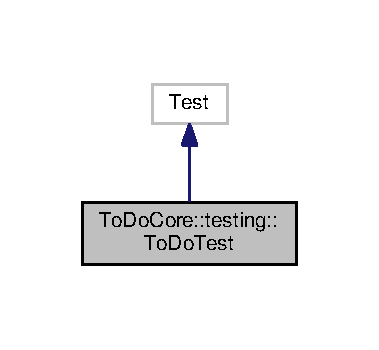
\includegraphics[width=182pt]{class_to_do_core_1_1testing_1_1_to_do_test__inherit__graph}
\end{center}
\end{figure}


Graphe de collaboration de To\+Do\+Core\+:\+:testing\+:\+:To\+Do\+Test\+:
\nopagebreak
\begin{figure}[H]
\begin{center}
\leavevmode
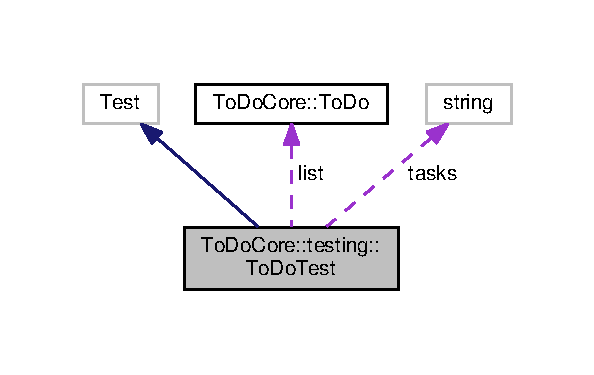
\includegraphics[width=285pt]{class_to_do_core_1_1testing_1_1_to_do_test__coll__graph}
\end{center}
\end{figure}
\subsection*{Fonctions membres protégées}
\begin{DoxyCompactItemize}
\item 
\hyperlink{class_to_do_core_1_1testing_1_1_to_do_test_ae616fd99cc5a805ca5e7dfd01161f838}{To\+Do\+Test} ()
\item 
\hyperlink{class_to_do_core_1_1testing_1_1_to_do_test_a60215b4387d7543fe3d8b95a4ea68efb}{$\sim$\+To\+Do\+Test} ()
\item 
virtual void \hyperlink{class_to_do_core_1_1testing_1_1_to_do_test_a7c6934ff5c428bbf570ba84a236c8ea8}{Set\+Up} ()
\item 
virtual void \hyperlink{class_to_do_core_1_1testing_1_1_to_do_test_a20a3f1fa62263094c32fed4460592a16}{Tear\+Down} ()
\end{DoxyCompactItemize}
\subsection*{Attributs protégés}
\begin{DoxyCompactItemize}
\item 
\hyperlink{class_to_do_core_1_1_to_do}{To\+Do} \hyperlink{class_to_do_core_1_1testing_1_1_to_do_test_aa574f1ef8dce28e299d993d06a0bbba9}{list}
\end{DoxyCompactItemize}
\subsection*{Attributs protégés statiques}
\begin{DoxyCompactItemize}
\item 
static const size\+\_\+t \hyperlink{class_to_do_core_1_1testing_1_1_to_do_test_a9f8905b1176e6183f287ab0afe296a3c}{task\+Count} = 3
\item 
static const string \hyperlink{class_to_do_core_1_1testing_1_1_to_do_test_a6ef770d8f95f609e100d585c0635f3d7}{tasks} \mbox{[}\hyperlink{class_to_do_core_1_1testing_1_1_to_do_test_a9f8905b1176e6183f287ab0afe296a3c}{task\+Count}\mbox{]} = \{\char`\"{}write code\char`\"{}, \char`\"{}compile\char`\"{}, \char`\"{}test\char`\"{}\}
\end{DoxyCompactItemize}


\subsection{Description détaillée}


Définition à la ligne 17 du fichier To\+Do\+Test.\+cc.



\subsection{Documentation des constructeurs et destructeur}
\hypertarget{class_to_do_core_1_1testing_1_1_to_do_test_ae616fd99cc5a805ca5e7dfd01161f838}{\index{To\+Do\+Core\+::testing\+::\+To\+Do\+Test@{To\+Do\+Core\+::testing\+::\+To\+Do\+Test}!To\+Do\+Test@{To\+Do\+Test}}
\index{To\+Do\+Test@{To\+Do\+Test}!To\+Do\+Core\+::testing\+::\+To\+Do\+Test@{To\+Do\+Core\+::testing\+::\+To\+Do\+Test}}
\subsubsection[{To\+Do\+Test}]{\setlength{\rightskip}{0pt plus 5cm}To\+Do\+Core\+::testing\+::\+To\+Do\+Test\+::\+To\+Do\+Test (
\begin{DoxyParamCaption}
{}
\end{DoxyParamCaption}
)\hspace{0.3cm}{\ttfamily [inline]}, {\ttfamily [protected]}}}\label{class_to_do_core_1_1testing_1_1_to_do_test_ae616fd99cc5a805ca5e7dfd01161f838}


Définition à la ligne 23 du fichier To\+Do\+Test.\+cc.

\hypertarget{class_to_do_core_1_1testing_1_1_to_do_test_a60215b4387d7543fe3d8b95a4ea68efb}{\index{To\+Do\+Core\+::testing\+::\+To\+Do\+Test@{To\+Do\+Core\+::testing\+::\+To\+Do\+Test}!````~To\+Do\+Test@{$\sim$\+To\+Do\+Test}}
\index{````~To\+Do\+Test@{$\sim$\+To\+Do\+Test}!To\+Do\+Core\+::testing\+::\+To\+Do\+Test@{To\+Do\+Core\+::testing\+::\+To\+Do\+Test}}
\subsubsection[{$\sim$\+To\+Do\+Test}]{\setlength{\rightskip}{0pt plus 5cm}To\+Do\+Core\+::testing\+::\+To\+Do\+Test\+::$\sim$\+To\+Do\+Test (
\begin{DoxyParamCaption}
{}
\end{DoxyParamCaption}
)\hspace{0.3cm}{\ttfamily [inline]}, {\ttfamily [protected]}}}\label{class_to_do_core_1_1testing_1_1_to_do_test_a60215b4387d7543fe3d8b95a4ea68efb}


Définition à la ligne 28 du fichier To\+Do\+Test.\+cc.



\subsection{Documentation des fonctions membres}
\hypertarget{class_to_do_core_1_1testing_1_1_to_do_test_a7c6934ff5c428bbf570ba84a236c8ea8}{\index{To\+Do\+Core\+::testing\+::\+To\+Do\+Test@{To\+Do\+Core\+::testing\+::\+To\+Do\+Test}!Set\+Up@{Set\+Up}}
\index{Set\+Up@{Set\+Up}!To\+Do\+Core\+::testing\+::\+To\+Do\+Test@{To\+Do\+Core\+::testing\+::\+To\+Do\+Test}}
\subsubsection[{Set\+Up}]{\setlength{\rightskip}{0pt plus 5cm}virtual void To\+Do\+Core\+::testing\+::\+To\+Do\+Test\+::\+Set\+Up (
\begin{DoxyParamCaption}
{}
\end{DoxyParamCaption}
)\hspace{0.3cm}{\ttfamily [inline]}, {\ttfamily [protected]}, {\ttfamily [virtual]}}}\label{class_to_do_core_1_1testing_1_1_to_do_test_a7c6934ff5c428bbf570ba84a236c8ea8}


Définition à la ligne 34 du fichier To\+Do\+Test.\+cc.

\hypertarget{class_to_do_core_1_1testing_1_1_to_do_test_a20a3f1fa62263094c32fed4460592a16}{\index{To\+Do\+Core\+::testing\+::\+To\+Do\+Test@{To\+Do\+Core\+::testing\+::\+To\+Do\+Test}!Tear\+Down@{Tear\+Down}}
\index{Tear\+Down@{Tear\+Down}!To\+Do\+Core\+::testing\+::\+To\+Do\+Test@{To\+Do\+Core\+::testing\+::\+To\+Do\+Test}}
\subsubsection[{Tear\+Down}]{\setlength{\rightskip}{0pt plus 5cm}virtual void To\+Do\+Core\+::testing\+::\+To\+Do\+Test\+::\+Tear\+Down (
\begin{DoxyParamCaption}
{}
\end{DoxyParamCaption}
)\hspace{0.3cm}{\ttfamily [inline]}, {\ttfamily [protected]}, {\ttfamily [virtual]}}}\label{class_to_do_core_1_1testing_1_1_to_do_test_a20a3f1fa62263094c32fed4460592a16}


Définition à la ligne 39 du fichier To\+Do\+Test.\+cc.



\subsection{Documentation des données membres}
\hypertarget{class_to_do_core_1_1testing_1_1_to_do_test_aa574f1ef8dce28e299d993d06a0bbba9}{\index{To\+Do\+Core\+::testing\+::\+To\+Do\+Test@{To\+Do\+Core\+::testing\+::\+To\+Do\+Test}!list@{list}}
\index{list@{list}!To\+Do\+Core\+::testing\+::\+To\+Do\+Test@{To\+Do\+Core\+::testing\+::\+To\+Do\+Test}}
\subsubsection[{list}]{\setlength{\rightskip}{0pt plus 5cm}{\bf To\+Do} To\+Do\+Core\+::testing\+::\+To\+Do\+Test\+::list\hspace{0.3cm}{\ttfamily [protected]}}}\label{class_to_do_core_1_1testing_1_1_to_do_test_aa574f1ef8dce28e299d993d06a0bbba9}
T\+O\+D\+O 

Définition à la ligne 41 du fichier To\+Do\+Test.\+cc.

\hypertarget{class_to_do_core_1_1testing_1_1_to_do_test_a9f8905b1176e6183f287ab0afe296a3c}{\index{To\+Do\+Core\+::testing\+::\+To\+Do\+Test@{To\+Do\+Core\+::testing\+::\+To\+Do\+Test}!task\+Count@{task\+Count}}
\index{task\+Count@{task\+Count}!To\+Do\+Core\+::testing\+::\+To\+Do\+Test@{To\+Do\+Core\+::testing\+::\+To\+Do\+Test}}
\subsubsection[{task\+Count}]{\setlength{\rightskip}{0pt plus 5cm}const size\+\_\+t To\+Do\+Core\+::testing\+::\+To\+Do\+Test\+::task\+Count = 3\hspace{0.3cm}{\ttfamily [static]}, {\ttfamily [protected]}}}\label{class_to_do_core_1_1testing_1_1_to_do_test_a9f8905b1176e6183f287ab0afe296a3c}
T\+O\+D\+O 

Définition à la ligne 43 du fichier To\+Do\+Test.\+cc.

\hypertarget{class_to_do_core_1_1testing_1_1_to_do_test_a6ef770d8f95f609e100d585c0635f3d7}{\index{To\+Do\+Core\+::testing\+::\+To\+Do\+Test@{To\+Do\+Core\+::testing\+::\+To\+Do\+Test}!tasks@{tasks}}
\index{tasks@{tasks}!To\+Do\+Core\+::testing\+::\+To\+Do\+Test@{To\+Do\+Core\+::testing\+::\+To\+Do\+Test}}
\subsubsection[{tasks}]{\setlength{\rightskip}{0pt plus 5cm}const string To\+Do\+Core\+::testing\+::\+To\+Do\+Test\+::tasks = \{\char`\"{}write code\char`\"{}, \char`\"{}compile\char`\"{}, \char`\"{}test\char`\"{}\}\hspace{0.3cm}{\ttfamily [static]}, {\ttfamily [protected]}}}\label{class_to_do_core_1_1testing_1_1_to_do_test_a6ef770d8f95f609e100d585c0635f3d7}
T\+O\+D\+O 

Définition à la ligne 44 du fichier To\+Do\+Test.\+cc.



La documentation de cette classe a été générée à partir du fichier suivant \+:\begin{DoxyCompactItemize}
\item 
/home/latty/\+Prog/\+C\+Make\+\_\+\+Tutorial/chapter\+\_\+4/src/\+To\+Do\+Core/unit\+\_\+test/\hyperlink{_to_do_test_8cc}{To\+Do\+Test.\+cc}\end{DoxyCompactItemize}

\chapter{Documentation des fichiers}
\hypertarget{main_8cc}{\section{Référence du fichier /home/latty/\+Prog/\+C\+Make\+\_\+\+Tutorial/chapter\+\_\+4/src/main.cc}
\label{main_8cc}\index{/home/latty/\+Prog/\+C\+Make\+\_\+\+Tutorial/chapter\+\_\+4/src/main.\+cc@{/home/latty/\+Prog/\+C\+Make\+\_\+\+Tutorial/chapter\+\_\+4/src/main.\+cc}}
}
{\ttfamily \#include $<$iostream$>$}\\*
{\ttfamily \#include \char`\"{}To\+Do\+Core/\+To\+Do.\+h\char`\"{}}\\*
Graphe des dépendances par inclusion de main.\+cc\+:\nopagebreak
\begin{figure}[H]
\begin{center}
\leavevmode
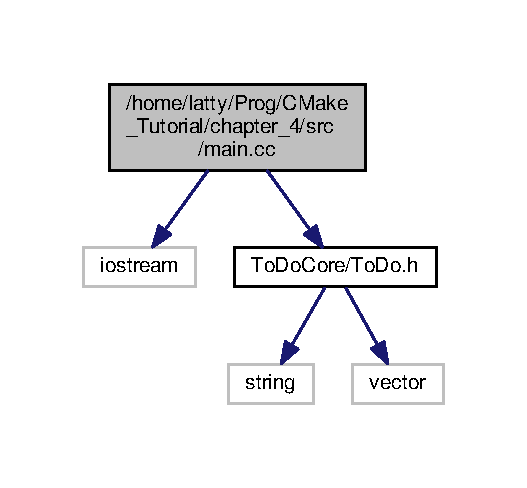
\includegraphics[width=253pt]{main_8cc__incl}
\end{center}
\end{figure}
\subsection*{Macros}
\begin{DoxyCompactItemize}
\item 
\#define \hyperlink{main_8cc_ab587f50c3683eb7b54ee78e460b7f349}{E\+X\+P\+E\+C\+T\+\_\+\+E\+Q\+U\+A\+L}(test, expect)
\end{DoxyCompactItemize}
\subsection*{Fonctions}
\begin{DoxyCompactItemize}
\item 
{\footnotesize template$<$typename T1 , typename T2 $>$ }\\int \hyperlink{main_8cc_a0f5bd42dc84b969c014e7b099e4ddff5}{equality\+Test} (const T1 test\+Value, const T2 expected\+Value, const char $\ast$test\+Name, const char $\ast$expected\+Name, const char $\ast$file\+Name, const int line\+Number)
\item 
int \hyperlink{main_8cc_a2c3f6775325c30275d11c6abee2db6a0}{main} (int, char $\ast$$\ast$)
\end{DoxyCompactItemize}


\subsection{Documentation des macros}
\hypertarget{main_8cc_ab587f50c3683eb7b54ee78e460b7f349}{\index{main.\+cc@{main.\+cc}!E\+X\+P\+E\+C\+T\+\_\+\+E\+Q\+U\+A\+L@{E\+X\+P\+E\+C\+T\+\_\+\+E\+Q\+U\+A\+L}}
\index{E\+X\+P\+E\+C\+T\+\_\+\+E\+Q\+U\+A\+L@{E\+X\+P\+E\+C\+T\+\_\+\+E\+Q\+U\+A\+L}!main.\+cc@{main.\+cc}}
\subsubsection[{E\+X\+P\+E\+C\+T\+\_\+\+E\+Q\+U\+A\+L}]{\setlength{\rightskip}{0pt plus 5cm}\#define E\+X\+P\+E\+C\+T\+\_\+\+E\+Q\+U\+A\+L(
\begin{DoxyParamCaption}
\item[{}]{test, }
\item[{}]{expect}
\end{DoxyParamCaption}
)}}\label{main_8cc_ab587f50c3683eb7b54ee78e460b7f349}
{\bfseries Valeur \+:}
\begin{DoxyCode}
\hyperlink{main_8cc_a0f5bd42dc84b969c014e7b099e4ddff5}{equalityTest}( test,  expect, \(\backslash\)
                                                #test, #expect, \(\backslash\)
                                                \_\_FILE\_\_, \_\_LINE\_\_)
\end{DoxyCode}


Définition à la ligne 9 du fichier main.\+cc.



\subsection{Documentation des fonctions}
\hypertarget{main_8cc_a0f5bd42dc84b969c014e7b099e4ddff5}{\index{main.\+cc@{main.\+cc}!equality\+Test@{equality\+Test}}
\index{equality\+Test@{equality\+Test}!main.\+cc@{main.\+cc}}
\subsubsection[{equality\+Test}]{\setlength{\rightskip}{0pt plus 5cm}template$<$typename T1 , typename T2 $>$ int equality\+Test (
\begin{DoxyParamCaption}
\item[{const T1}]{test\+Value, }
\item[{const T2}]{expected\+Value, }
\item[{const char $\ast$}]{test\+Name, }
\item[{const char $\ast$}]{expected\+Name, }
\item[{const char $\ast$}]{file\+Name, }
\item[{const int}]{line\+Number}
\end{DoxyParamCaption}
)}}\label{main_8cc_a0f5bd42dc84b969c014e7b099e4ddff5}

\begin{DoxyParams}{Paramètres}
{\em test\+Value} & \\
\hline
{\em expected\+Value} & \\
\hline
{\em test\+Name} & \\
\hline
{\em expected\+Name} & \\
\hline
{\em file\+Name} & \\
\hline
{\em line\+Number} & \\
\hline
\end{DoxyParams}
\begin{DoxyReturn}{Renvoie}
int 
\end{DoxyReturn}


Définition à la ligne 79 du fichier main.\+cc.

\hypertarget{main_8cc_a2c3f6775325c30275d11c6abee2db6a0}{\index{main.\+cc@{main.\+cc}!main@{main}}
\index{main@{main}!main.\+cc@{main.\+cc}}
\subsubsection[{main}]{\setlength{\rightskip}{0pt plus 5cm}int main (
\begin{DoxyParamCaption}
\item[{int}]{, }
\item[{char $\ast$$\ast$}]{}
\end{DoxyParamCaption}
)}}\label{main_8cc_a2c3f6775325c30275d11c6abee2db6a0}

\begin{DoxyParams}{Paramètres}
{\em int} & \\
\hline
{\em } & return int \\
\hline
\end{DoxyParams}


Définition à la ligne 40 du fichier main.\+cc.


\hypertarget{_to_do_8cc}{\section{Référence du fichier /home/latty/\+Prog/\+C\+Make\+\_\+\+Tutorial/chapter\+\_\+4/src/\+To\+Do\+Core/\+To\+Do.cc}
\label{_to_do_8cc}\index{/home/latty/\+Prog/\+C\+Make\+\_\+\+Tutorial/chapter\+\_\+4/src/\+To\+Do\+Core/\+To\+Do.\+cc@{/home/latty/\+Prog/\+C\+Make\+\_\+\+Tutorial/chapter\+\_\+4/src/\+To\+Do\+Core/\+To\+Do.\+cc}}
}
{\ttfamily \#include \char`\"{}To\+Do.\+h\char`\"{}}\\*
Graphe des dépendances par inclusion de To\+Do.\+cc\+:
\nopagebreak
\begin{figure}[H]
\begin{center}
\leavevmode
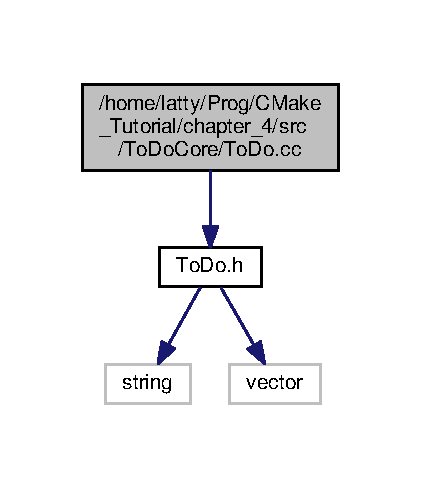
\includegraphics[width=202pt]{_to_do_8cc__incl}
\end{center}
\end{figure}
\subsection*{Espaces de nommage}
\begin{DoxyCompactItemize}
\item 
 \hyperlink{namespace_to_do_core}{To\+Do\+Core}
\end{DoxyCompactItemize}

\hypertarget{_to_do_8h}{\section{Référence du fichier /home/latty/\+Prog/\+C\+Make\+\_\+\+Tutorial/chapter\+\_\+4/src/\+To\+Do\+Core/\+To\+Do.h}
\label{_to_do_8h}\index{/home/latty/\+Prog/\+C\+Make\+\_\+\+Tutorial/chapter\+\_\+4/src/\+To\+Do\+Core/\+To\+Do.\+h@{/home/latty/\+Prog/\+C\+Make\+\_\+\+Tutorial/chapter\+\_\+4/src/\+To\+Do\+Core/\+To\+Do.\+h}}
}
{\ttfamily \#include $<$string$>$}\\*
{\ttfamily \#include $<$vector$>$}\\*
Graphe des dépendances par inclusion de To\+Do.\+h\+:\nopagebreak
\begin{figure}[H]
\begin{center}
\leavevmode
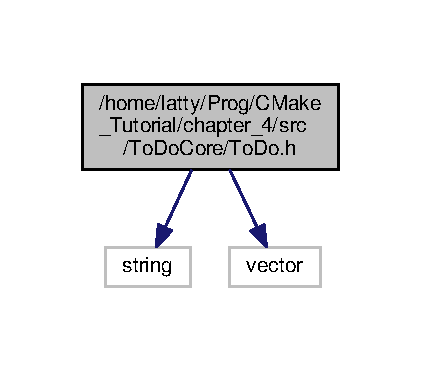
\includegraphics[width=202pt]{_to_do_8h__incl}
\end{center}
\end{figure}
Ce graphe montre quels fichiers incluent directement ou indirectement ce fichier \+:\nopagebreak
\begin{figure}[H]
\begin{center}
\leavevmode
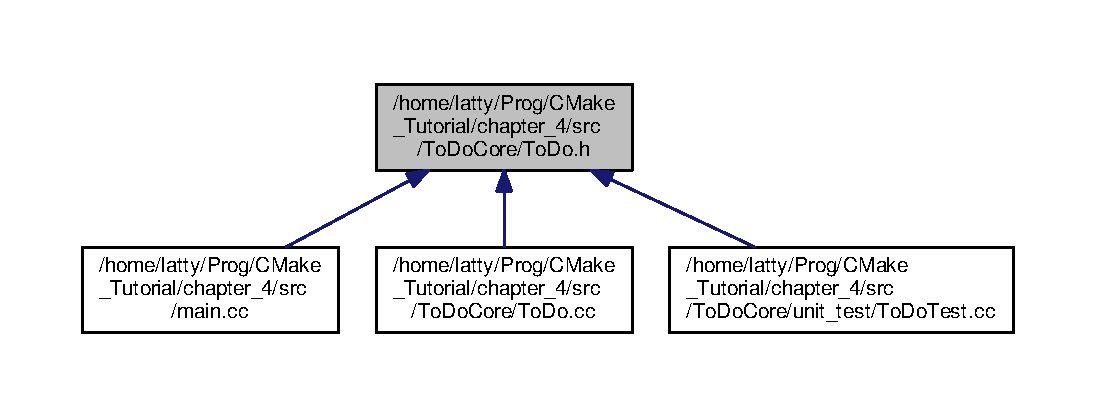
\includegraphics[width=350pt]{_to_do_8h__dep__incl}
\end{center}
\end{figure}
\subsection*{Classes}
\begin{DoxyCompactItemize}
\item 
class \hyperlink{class_to_do_core_1_1_to_do}{To\+Do\+Core\+::\+To\+Do}
\end{DoxyCompactItemize}
\subsection*{Espaces de nommage}
\begin{DoxyCompactItemize}
\item 
 \hyperlink{namespace_to_do_core}{To\+Do\+Core}
\end{DoxyCompactItemize}

\hypertarget{_to_do_test_8cc}{\section{Référence du fichier /home/latty/\+Prog/\+C\+Make\+\_\+\+Tutorial/chapter\+\_\+4/src/\+To\+Do\+Core/unit\+\_\+test/\+To\+Do\+Test.cc}
\label{_to_do_test_8cc}\index{/home/latty/\+Prog/\+C\+Make\+\_\+\+Tutorial/chapter\+\_\+4/src/\+To\+Do\+Core/unit\+\_\+test/\+To\+Do\+Test.\+cc@{/home/latty/\+Prog/\+C\+Make\+\_\+\+Tutorial/chapter\+\_\+4/src/\+To\+Do\+Core/unit\+\_\+test/\+To\+Do\+Test.\+cc}}
}
{\ttfamily \#include \char`\"{}To\+Do\+Core/\+To\+Do.\+h\char`\"{}}\\*
{\ttfamily \#include $<$string$>$}\\*
{\ttfamily \#include $<$gmock/gmock.\+h$>$}\\*
{\ttfamily \#include $<$gtest/gtest.\+h$>$}\\*
Graphe des dépendances par inclusion de To\+Do\+Test.\+cc\+:\nopagebreak
\begin{figure}[H]
\begin{center}
\leavevmode
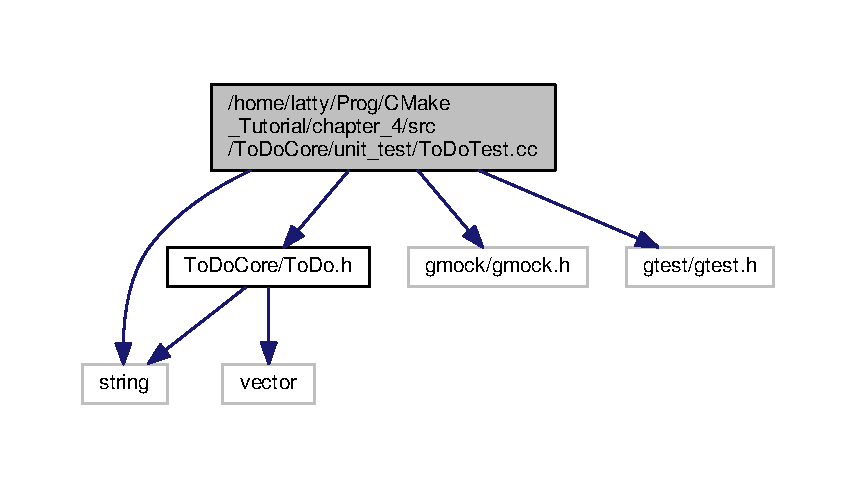
\includegraphics[width=350pt]{_to_do_test_8cc__incl}
\end{center}
\end{figure}
\subsection*{Classes}
\begin{DoxyCompactItemize}
\item 
class \hyperlink{class_to_do_core_1_1testing_1_1_to_do_test}{To\+Do\+Core\+::testing\+::\+To\+Do\+Test}
\end{DoxyCompactItemize}
\subsection*{Espaces de nommage}
\begin{DoxyCompactItemize}
\item 
 \hyperlink{namespace_to_do_core}{To\+Do\+Core}
\item 
 \hyperlink{namespace_to_do_core_1_1testing}{To\+Do\+Core\+::testing}
\end{DoxyCompactItemize}
\subsection*{Fonctions}
\begin{DoxyCompactItemize}
\item 
\hyperlink{namespace_to_do_core_1_1testing_a8856a84197dfa84ec81d14bd227c2264}{To\+Do\+Core\+::testing\+::\+T\+E\+S\+T\+\_\+\+F} (To\+Do\+Test, constructor\+\_\+creates\+Empty\+List)
\item 
\hyperlink{namespace_to_do_core_1_1testing_ad1ff01cd7b75e9ba48225bbde5f1bb2b}{To\+Do\+Core\+::testing\+::\+T\+E\+S\+T\+\_\+\+F} (To\+Do\+Test, add\+Task\+\_\+three\+Times\+\_\+size\+Is\+Three)
\item 
\hyperlink{namespace_to_do_core_1_1testing_a8d6cdf71a6d2d85a7d6dc6e4ced72c51}{To\+Do\+Core\+::testing\+::\+T\+E\+S\+T\+\_\+\+F} (To\+Do\+Test, get\+Task\+\_\+with\+One\+Task\+\_\+returns\+Correct\+String)
\item 
\hyperlink{namespace_to_do_core_1_1testing_ae6f99ee22a68254ccf5750d1788cd082}{To\+Do\+Core\+::testing\+::\+T\+E\+S\+T\+\_\+\+F} (To\+Do\+Test, get\+Task\+\_\+with\+Three\+Tasts\+\_\+returns\+Correct\+String\+For\+Each\+Index)
\end{DoxyCompactItemize}

%--- End generated contents ---

% Index
\newpage
\phantomsection
\addcontentsline{toc}{chapter}{Index}
\printindex

\end{document}
